%package list
\documentclass[]{article}
\usepackage[top=3cm, bottom=3cm, outer=3cm, inner=3cm]{geometry}
\usepackage{graphicx}
\usepackage{url}
%\usepackage{cite}
\usepackage{hyperref}
\usepackage{array}
%\usepackage{multicol}
\newcolumntype{x}[1]{>{\centering\arraybackslash\hspace{0pt}}p{#1}}
\usepackage{natbib}
\usepackage{pdfpages}
\usepackage[export]{adjustbox}
% \usepackage{multirow}
\usepackage[T1]{fontenc}
\usepackage{imakeidx}
% Imagenes de costado
% \usepackage{wrapfig}
% \usepackage{graphicx}

% Modificar URLs
\usepackage{hyperref}
\hypersetup{
    colorlinks=true,
    linkcolor=black,
    filecolor=magenta,      
    urlcolor=blue,
    pdftitle={Overleaf Example},
    pdfpagemode=FullScreen,
    }

\urlstyle{same}


\usepackage[normalem]{ulem}
\useunder{\uline}{\ul}{}

\usepackage[newfloat]{minted}
\usepackage{caption}

\newenvironment{code}{\captionsetup{type=listing}}{}
\SetupFloatingEnvironment{listing}{name=Source Code}

% codigo fuente
\usepackage{listings}
\usepackage{color, colortbl}
\definecolor{dkgreen}{rgb}{0,0.6,0}
\definecolor{gray}{rgb}{0.5,0.5,0.5}
\definecolor{mauve}{rgb}{0.58,0,0.82}
\definecolor{codebackground}{rgb}{0.95, 0.95, 0.92}
\definecolor{tablebackground}{rgb}{0.0, 0.45, 0.63}
\lstset{frame=tb,
	language=bash,
	aboveskip=3mm,
	belowskip=3mm,
	showstringspaces=false,
	columns=flexible,
	basicstyle={\small\ttfamily},
	numbers=none,
	numberstyle=\tiny\color{gray},
	keywordstyle=\color{blue},
	commentstyle=\color{dkgreen},
	stringstyle=\color{mauve},
	breaklines=true,
	breakatwhitespace=true,
	tabsize=3,
	backgroundcolor= \color{codebackground},
}

%%%%%%%%%%%%%%%%%%%%%%%%%%%%%%%%%%%%%%%%%%%%%%%%%%%%%%%%%%%%%%%%%%%%%%%%%%%%
%%%%%%%%%%%%%%%%%%%%%%%%%%%%%%%%%%%%%%%%%%%%%%%%%%%%%%%%%%%%%%%%%%%%%%%%%%%%
\newcommand{\csemail}{pramirezs@ulasalle.edu.pe}
\newcommand{\csdocente}{MSc. Maribel Molina Barriga}
\newcommand{\cscurso}{Sistemas Operativos}
\newcommand{\csuniversidad}{Universidad La Salle}
\newcommand{\csescuela}{Escuela Profesional de Ingeniería de Software}
\newcommand{\cspracnr}{03}
\newcommand{\cstema}{Compilacion en C y C++ en Linux}
%%%%%%%%%%%%%%%%%%%%%%%%%%%%%%%%%%%%%%%%%%%%%%%%%%%%%%%%%%%%%%%%%%%%%%%%%%%%
%%%%%%%%%%%%%%%%%%%%%%%%%%%%%%%%%%%%%%%%%%%%%%%%%%%%%%%%%%%%%%%%%%%%%%%%%%%%


\usepackage[english,spanish]{babel}
\usepackage[utf8]{inputenc}
\AtBeginDocument{\selectlanguage{spanish}}
\renewcommand{\figurename}{Figura}
\renewcommand{\refname}{Referencias}
\renewcommand{\tablename}{Tabla} %esto no funciona cuando se usa babel
\AtBeginDocument{%
	\renewcommand\tablename{Tabla}
}

\usepackage{fancyhdr}
\pagestyle{fancy}
\fancyhf{}
\setlength{\headheight}{30pt}
\renewcommand{\headrulewidth}{1pt}
\renewcommand{\footrulewidth}{1pt}
\fancyhead[L]{\raisebox{-0.2\height}{
\includegraphics[width=3cm]{logo_ulasalle.png}}}
\fancyhead[C]{}
\fancyhead[R]{\fontsize{7}{7}\selectfont	\csuniversidad \\ \csescuela \\ \textbf{\cscurso} }
\fancyfoot[L]{}
\fancyfoot[C]{Sistemas Operativos}
\fancyfoot[R]{Página \thepage}



\begin{document}

	\vspace*{10px}
	
	\begin{center}	
		\fontsize{17}{17} \textbf{Practica \cspracnr}
	\end{center}
	%\centerline{\textbf{\underline{\Large Título: Informe de revisión del estado del arte}}}
	%\vspace*{0.5cm}
	

\renewcommand{\arraystretch}{1.5}
\begin{table}[h]
	\begin{tabular}{|x{4.7cm}|x{4.8cm}|x{4.8cm}|}
		\hline 
		\textbf{DOCENTE} & \textbf{CARRERA}  & \textbf{CURSO}   \\
		\hline 
		\csdocente & \csescuela & \cscurso    \\
		\hline 
	\end{tabular}
\end{table}	

\begin{table}[h]
	\begin{tabular}{|x{4.7cm}|x{4.8cm}|x{4.8cm}|}
		\hline 
		\textbf{GRUPO} & \textbf{TEMA}  & \textbf{DURACIÓN}   \\
		\hline 
		\ 6 & \cstema & 5 horas   \\
		\hline 
	\end{tabular}
\end{table}
\renewcommand{\arraystretch}{1} 
	\section*{Integrantes}
	 	\begin{itemize}
            \item José Carlos Machaca Vera
	 		\item Jhosep Alonso Mollapaza Morocco
	 		\item Patrick Andres Ramirez Santos
	 \end{itemize}
 
	\tableofcontents
\newpage

\section{Ejercicios propuestos}
Se deberá de probar, compilar y ejecutar los siguientes códigos:
\subsection{Ejercicio 1}
Se crea un archivo Cmake para facilitar la compilacion y ejecucion 
del codigo, este se presenta a continuacion, y que se puede utilizar 
con los siguientes comandos desde el directorio con los archivos:

\begin{minted}{bash}
	$ mkdir cmake-build-debug/
	$ cd cmake-build-debug/
	$ cmake .. # Buscar el archivo CMakeLists.txt en el directorio superior
	$ make # Compilar el proyecto
	$ ./E1 # Ejecutar el proyecto
\end{minted}

\begin{code}
	\captionof{listing}{Contenidos Makefile}
	\inputminted{cmake}{../E1/CMakeLists.txt}
\end{code}

\subsubsection*{proceso.cpp}
Este código crea un proceso hijo que imprime un mensaje en pantalla.
\begin{code}
	\captionof{listing}{Contenidos Makefile}
	\inputminted{c}{../E1/proceso.c}
\end{code}


\subsubsection*{ejemplo.cpp}
Este código utiliza polimorfismo para detectar el tipo de un objeto e imprimir
una funcion especifica en base a ello:
\begin{code}
	\captionof{listing}{Contenidos Makefile}
	\inputminted{c}{../E1/ejemplo.cpp}
\end{code}

\subsection{Ejercicio 2}
Este código recibe 2 argumentos vía línea de comandos, el primero es un 
número de segundos y el segundo es un mensaje, el código espera el tiempo
definido por el primer argumento y luego imprime el mensaje en pantalla 
de forma indefinida.
\begin{code}
	\captionof{listing}{E2/main.cpp}
	\inputminted{cpp}{../E2/main.cpp}
\end{code}

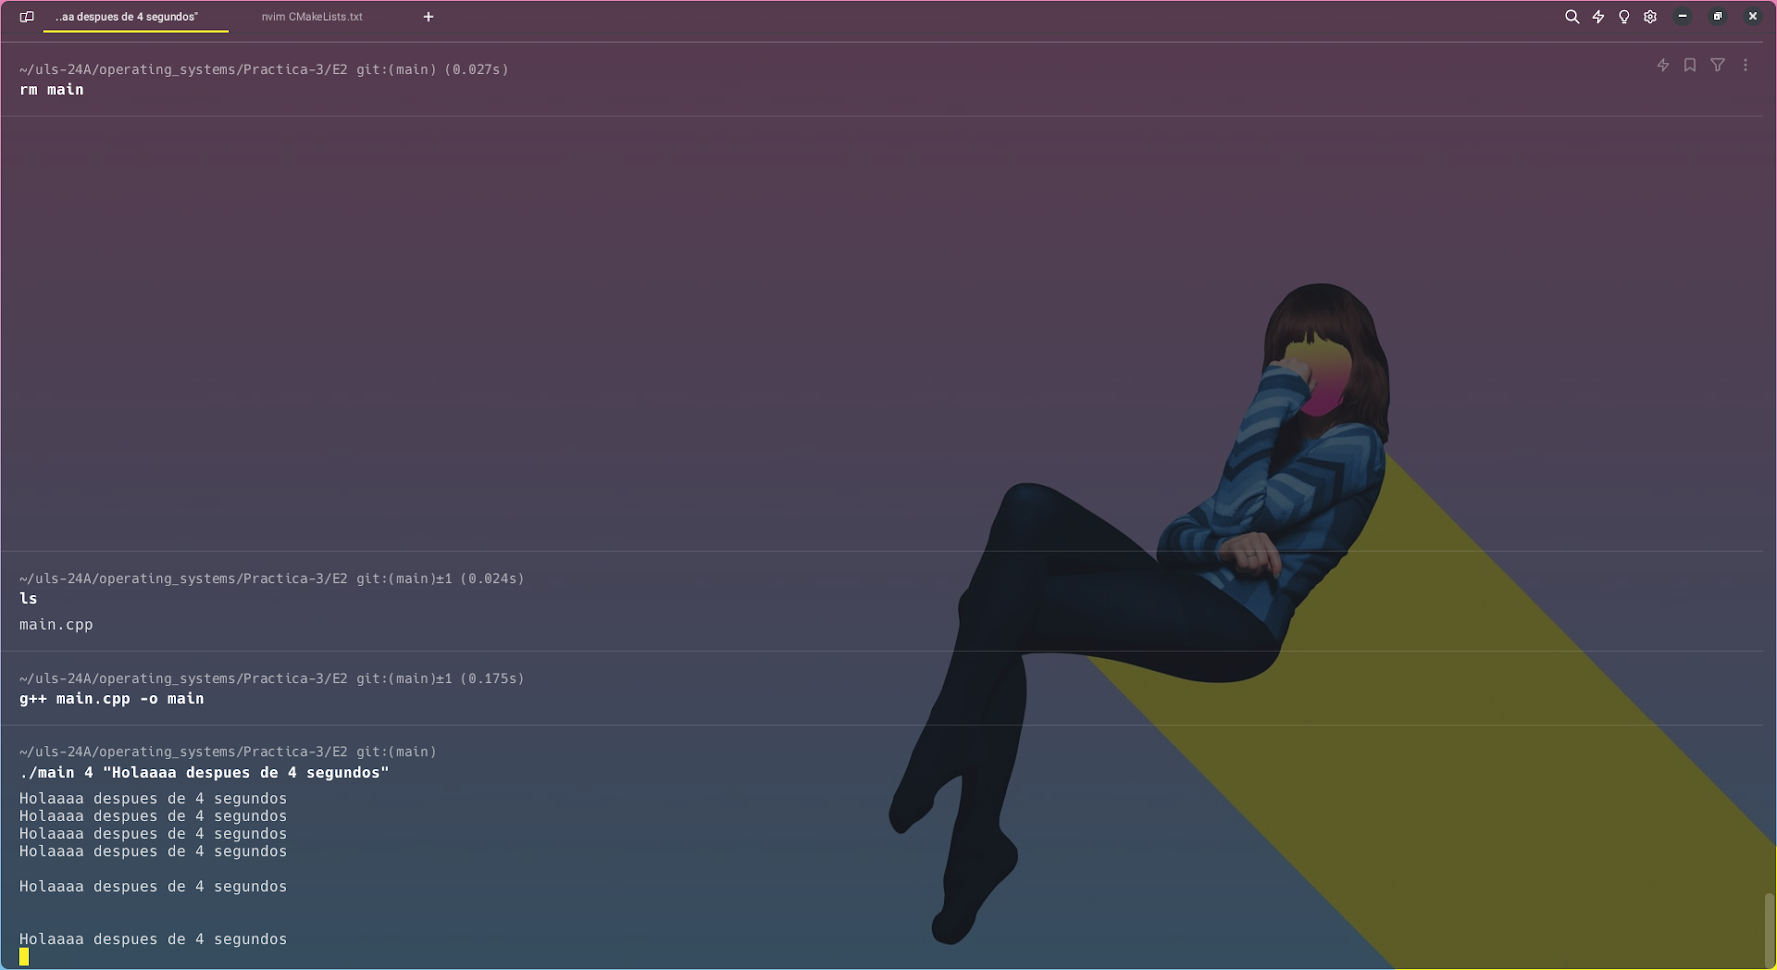
\includegraphics[scale=0.3,trim={0 0 20cm 20cm},clip]{e2-out.png}  

\subsection{Ejercicio 3}
En este ejercicio se utiliza un Makefile para compilar el archivo mensaje.c
y los archivos que este requiere para ejecutarse, para ejecutarlo se deben 
seguir los siguientes comandos, luego se muestra el contenido del Makefile:
\begin{minted}{bash}
	$ make # Compilar el proyecto con el makefile
	$ ./mensaje # Ejecutar el proyecto
\end{minted}

\begin{code}
	\captionof{listing}{E3/Makefile}
	\label{code:c-code}
	\inputminted{Makefile}{../E3/Makefile}
\end{code}
		
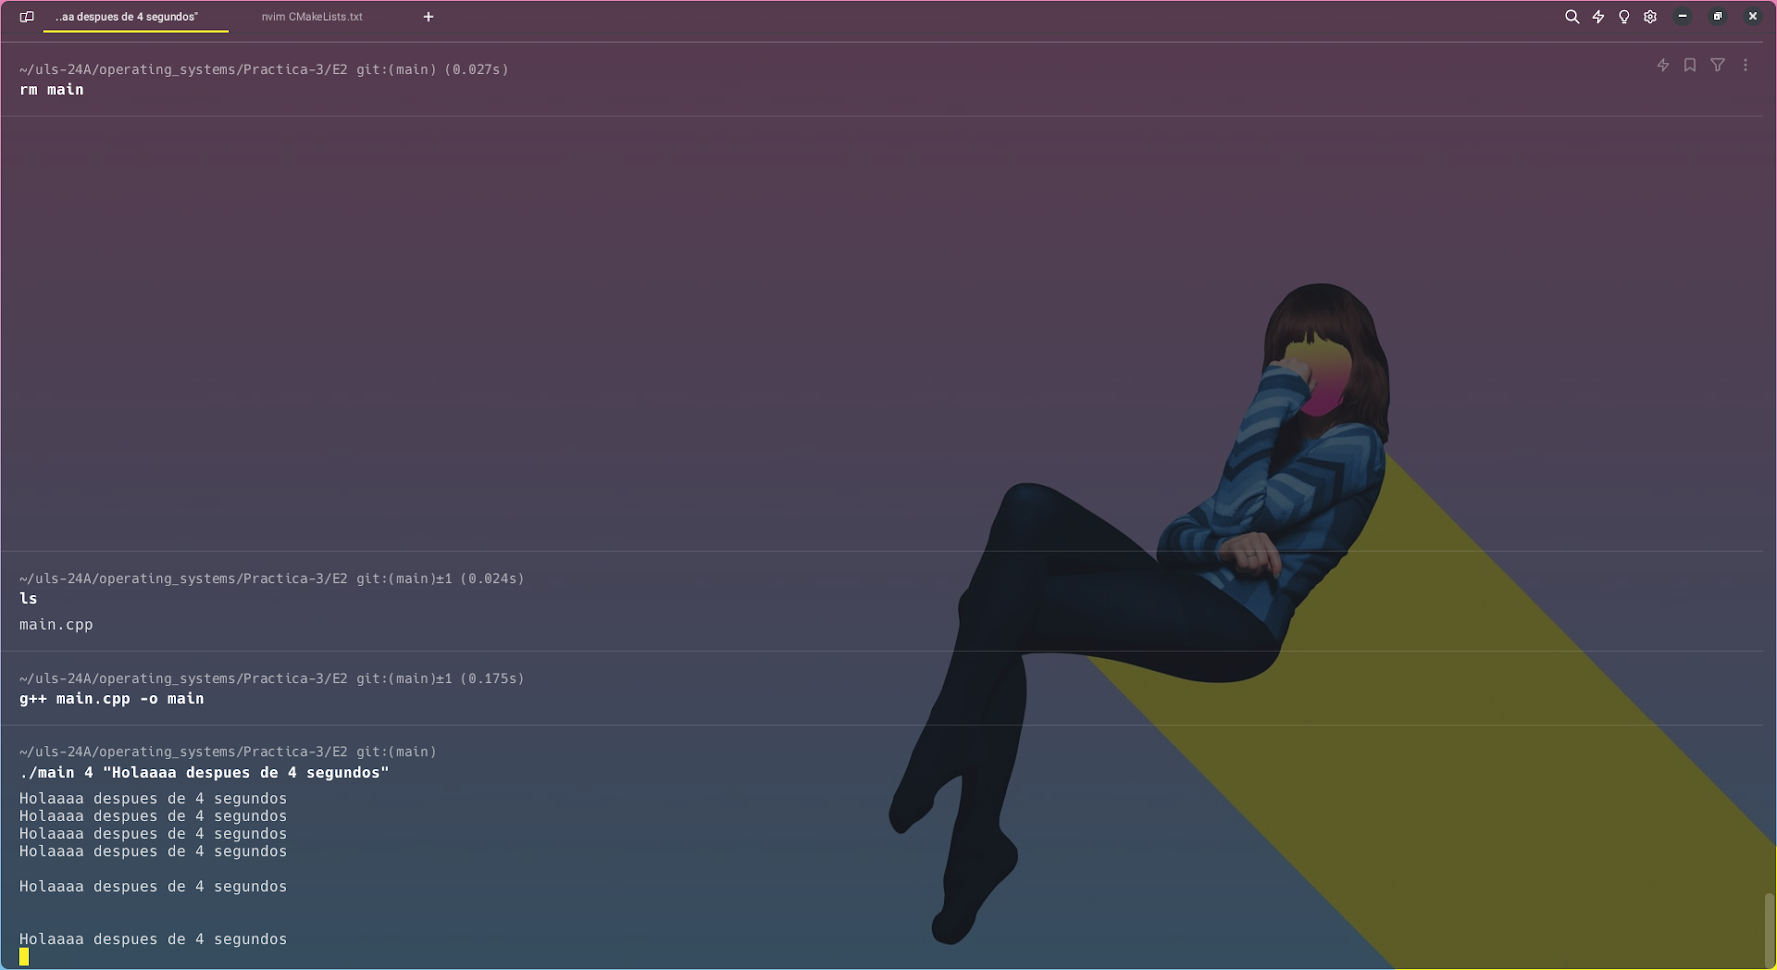
\includegraphics[scale=0.3,trim={0 0 20cm 20cm},clip]{e2-out.png}  


\section{Cuestionario}
\begin{enumerate}

	\item ¿Cuál es la diferencia entre compilar con GCC y G++? \\
	GCC es el compilador de GNU para C y otros lenguajes, mientras que G++ 
	es especificamente el compilador de GNU para C++. La principal diferencia
	 es en el lenguaje de programacion para el cual estan optimizados, ademas 
	 que G++ automaticamente vincula las bibliotecas estandar de C++ que no 
	 estan vinculadas por GCC

	\item ¿En que se diferencia el archivo generado .o contra un .exe

	\begin{itemize}
		\item Un archivo. o es un archivo de objeto, resultado de compilar 
		archivo de código fuente pero sin enlazarlo. Los archivos de objeto 
		contienen código máquina (binario), y no son ejecutables por sí mismos,
		ya que dependen de otros archivos.
		\item Un archivo .exe es un archivo ejecutable completo, resultado del 
		proceso  de enlazado de uno o varios archivos de objeto, junto con todas
		las bibliotecas necesarias para formar un programa que puede ser 
		ejecutado por el sistema operativo.
	\end{itemize}

	\item ¿Explique cuál es la diferencia entre el proceso de compilación y 
	enlazado? Proponga un ejemplo en haga uso de más de un archivo donde se 
	evidencie ambos procesos.
	\begin{itemize}
		\item La compilación es la conversión del código fuente a código objeto, 
		mientras que el enlazado es la unión de varios archivos de código objeto
		en un ejecutable.
		\item En el Ejemplo N°2 se puede ver cómo el Makefile enlaza varios 
		archivos para compilar correctamente el programa final.
	\end{itemize}
\end{enumerate}


        
\section{Conclusiones}
    \begin{itemize}
        \item Utilizando la salida de Valgrind, identificamos problemas críticos de manejo de memoria, como lecturas y liberaciones inválidas, y fugas de memoria relacionadas con las operaciones en tus clases ListNode y LinkedList.
        \item A través de los ejercicios realizados, se observó la importancia de la correcta utilización de las herramientas de compilación como GCC y G++ para manejar adecuadamente las dependencias y particularidades de cada lenguaje.
        \item La implementación de archivos CMakeLists.txt y Makefile en los ejercicios demostró cómo la automatización del proceso de compilación y enlazado mejora la eficiencia del desarrollo y permite una gestión más clara de los proyectos grandes.
        \item El manejo correcto de múltiples archivos en el proceso de compilación y enlazado fue crucial para la construcción exitosa de aplicaciones, destacando la importancia de entender ambos procesos para resolver dependencias y errores de enlazado.
    \end{itemize}

\section{Recomendaciones}
    \begin{itemize}
        \item Se sugirió evitar métodos recursivos de eliminación en estructuras de datos que potencialmente podrían ser muy largas para prevenir desbordamientos de pila.
Se enfatizó la importancia de asegurar que cada operación de new tenga su correspondiente delete para evitar fugas de memoria.
        \item  Es recomendable utilizar herramientas como CMake para gestionar proyectos más complejos, ya que simplifican y estandarizan el proceso de compilación y enlazado en diferentes entornos de desarrollo.
        \item Mantenerse actualizado sobre las mejores prácticas y nuevas características de las herramientas de compilación puede ayudar a optimizar el rendimiento y la eficiencia del código.
        \item Realizar pruebas exhaustivas durante y después del proceso de desarrollo para asegurarse de que el código funciona correctamente en diferentes plataformas y configuraciones de compilación.
	\end{itemize}

\renewcommand{\listlistingname}{Indice Source Code}
\listoflistings
\addcontentsline{toc}{section}{\listlistingname}

% \section{Cuadrilla KEKW}
%    \begin{tabular}{cc}
%        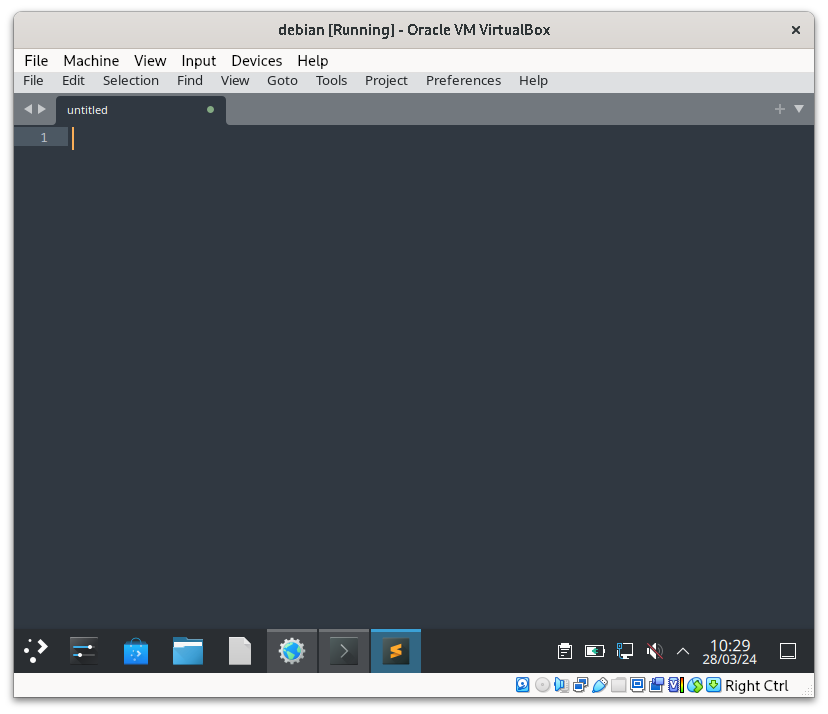
\includegraphics[width=.4\linewidth,valign=m]{capturas_paquetes/sublime.png} & 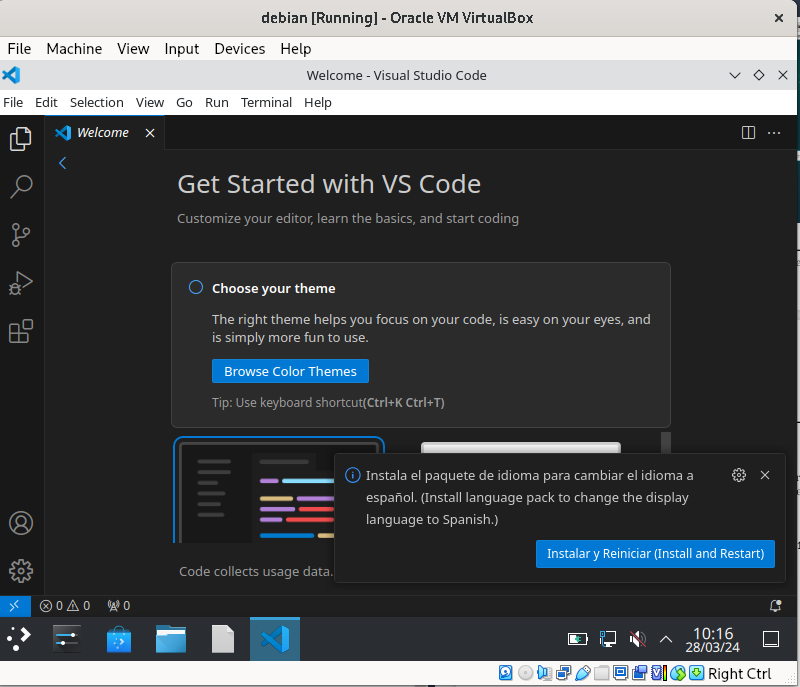
\includegraphics[width=.4\linewidth,valign=m]{capturas_paquetes/vscode.png} \\
%        Sublime & VS Code \\
%        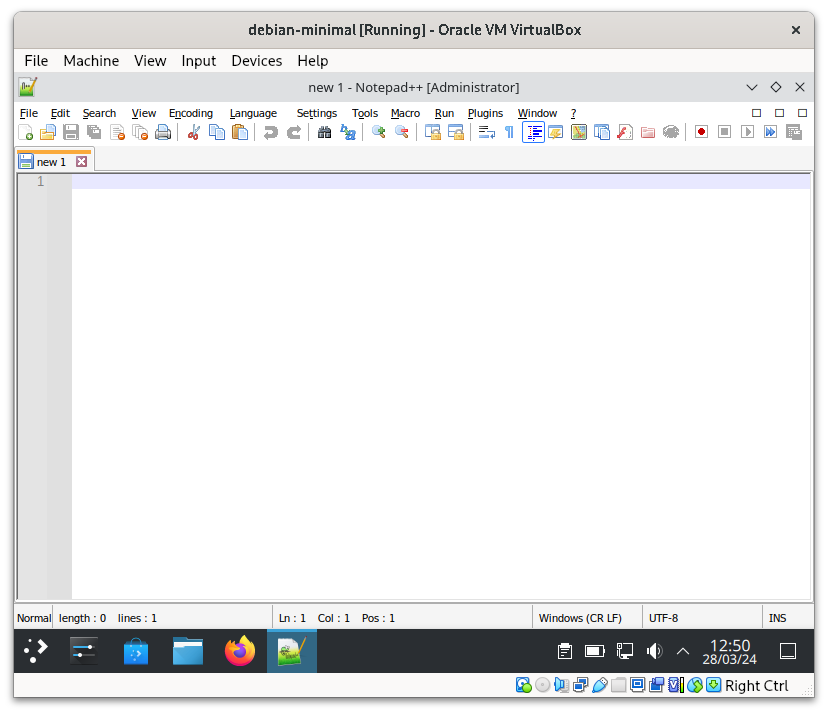
\includegraphics[width=.4\linewidth,valign=m]{capturas_paquetes/notepad.png} & 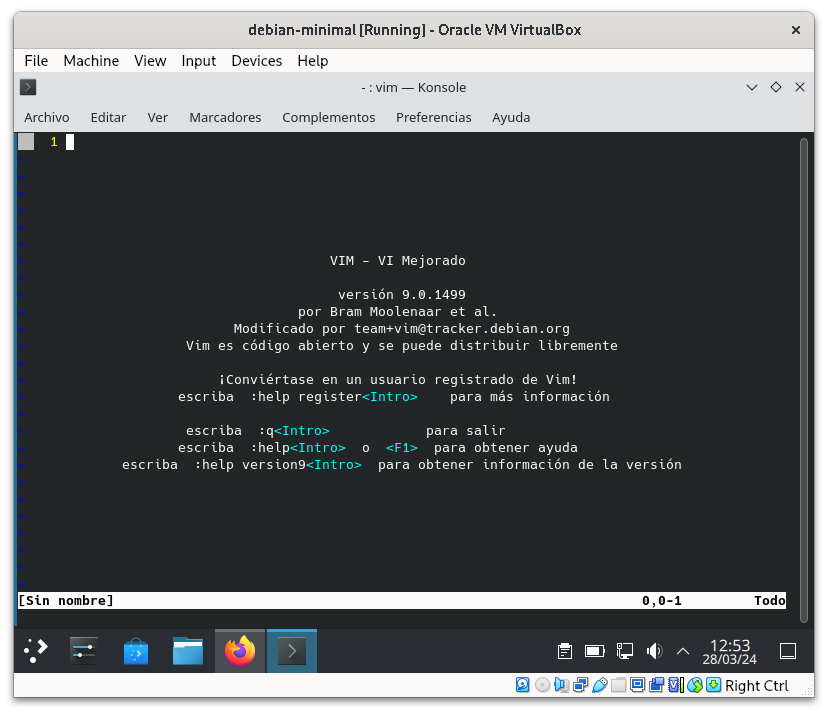
\includegraphics[width=.4\linewidth,valign=m]{capturas_paquetes/vim.png} \\
%        Notepad++ & Vim \\
%    \end{tabular}

	%\clearpage
	%\bibliographystyle{apalike}
	%\bibliographystyle{IEEEtranN}
	%\bibliography{bibliography}
		
	
\end{document}
